% =====================================================================
%  Professioni 5 — Il programmatore di videogiochi
%  Fonte: trascrizione della presentazione del corso di programmazione
%  ai Dev Days (AIV5): un incontro online su Zoom di circa un'ora e
%  mezza, in mattinata, tenuto da due docenti di programmazione di AIV,
%  Matteo Chironi (primo anno) ed Eugenio Fattori (secondo e terzo
%  anno). Circa 18-21 partecipanti di tutti i corsi; slide condivise;
%  lunga parte finale di domande.
%  Pacchetti richiesti nel preambolo del libro:
%    \usepackage[utf8]{inputenc}, \usepackage{booktabs},
%    \usepackage{amsmath},
%    \usepackage{tikz} con
%    \usetikzlibrary{arrows.meta,positioning,calc,fit}
%
%  Collocazione nel libro: parte "Alcune Professioni nel Mondo
%  Videoludico", dopo AIV4_character_animation (3.6).
%  Tutte le etichette di questo capitolo hanno il prefisso "p5:".
% =====================================================================

\chapter[Il programmatore di videogiochi]{Il programmatore di videogiochi:
specializzazioni, comunicazione e ``fame''}
\label{p5:cap:programming}

La presentazione del corso di \textbf{programmazione} dei Dev Days
(capitolo~\ref{p1:cap:devdays}) è tenuta da due docenti:
\begin{itemize}
  \item \textbf{Eugenio Fattori}, docente del secondo e del terzo anno di
        programmazione, ex studente di AIV;
  \item \textbf{Matteo Chironi}, docente del primo anno dal 2007, che tiene la
        parte tecnica.
\end{itemize}
Come tutte le presentazioni della settimana, è pensata soprattutto per chi
\textbf{non} farà programmazione: in apertura Fattori chiede quanti
programmatori ci siano (``una buonissima percentuale, direi. Che cazzo mi fate
qua? Vabbè, battute a parte'') e constata che il pubblico è fatto in parte di
designer, in parte di 3D artist, con qualche narrative. Per questo chiede a
Chironi di fare ``una roba un po' più soft'', ``perché probabilmente dei
dettagli tecnici vi interessa il giusto''; e Chironi promette di fare la
parte tecnica ``veloce'', ``giusto per farvi capire cosa sono gli uni e gli
zeri quando vedete al telegiornale hackerato il coso'', lasciando spazio alle
domande. Fra gli iscritti a programmazione presenti ci sono Giordano (``mi sa
che gli avevo già fatto il colloquio'') e Matteo; Filippo è di game design ma
``sotto sotto'' interessato.

L'incontro si tiene online, in mattinata (``volevo testare il livello di
dormienza a quest'ora''); i partecipanti salgono da 18 a 21. La data non è
detta; un indizio la colloca con ogni probabilità \textbf{mercoledì 7 ottobre
2026}\footnote{Uno studente dice di aver fatto la stessa domanda ``ieri al
professore di narrative design'', e la presentazione di narrative si è tenuta
martedì 6 ottobre (capitolo~\ref{p3:cap:narrative}). Verso la fine, però, un
altro studente dice che la webcam ``mi arriva il 6 ottobre'', come se la data
fosse ancora futura: le due cose non sono compatibili, e una delle due è con
ogni probabilità trascritta male. La Milan Games Week, citata ``fra un mese e
mezzo'', si tiene di solito fra la fine di novembre e l'inizio di dicembre:
l'indizio è compatibile con inizio ottobre.}.

Avvertenza di lettura: la trascrizione è automatica e particolarmente
disturbata. Si apre con un lungo blocco allucinato dal software (``la
risposta è la stessa'' ripetuto decine di volte, frasi su ``la signora
Nicolai Katainen'', ``la Corte Suprema di Internet'', ``la loro dottrina sul
mercato del lavoro''), qui ignorato. Non distingue i due relatori: le
attribuzioni sono ricostruite dal contesto (Chironi presenta le slide e fa il
primo anno; Fattori ha lavorato in Sumo Digital e farà il secondo e il terzo
anno) e, dove restano dubbie, lo si segnala. Storpia molti nomi: AIV diventa
``Hive'' e ``live''; Unreal ``Real Engine'' e ``a Real''; C\# e C++ diventano
semplicemente ``C''; la First Playable di Firenze ``Firenze necessaria''. Le
slide di Chironi, dice lui stesso, erano state preparate ``un po' di anni fa,
quando andavamo nelle scuole a far vedere che nei videogiochi c'era la
matematica, la fisica''; alcuni passaggi semplificano molto, e alcune
affermazioni sono inesatte: lo si segnala in nota.

Il percorso del capitolo:
\begin{enumerate}
  \item i relatori e il corso (sezione~\ref{p5:sec:corso});
  \item come funziona un computer: binario, hardware, software, compilatore
        (sezione~\ref{p5:sec:computer});
  \item le \textbf{specializzazioni}: rendering, fisica, gameplay,
        intelligenza artificiale, networking
        (sezioni da~\ref{p5:sec:specializzazioni} a~\ref{p5:sec:network});
  \item che cosa fa, in sintesi, il programmatore (sezione~\ref{p5:sec:ruolo});
  \item \textbf{come si comunica con un programmatore}
        (sezione~\ref{p5:sec:comunicare});
  \item le domande: come prepararsi, la ``fame'', gli esami, l'IA, i libri, le
        attitudini, le fiere e le game jam
        (sezione~\ref{p5:sec:domande}).
\end{enumerate}

% ---------------------------------------------------------------------
\section{I relatori e il corso}
\label{p5:sec:corso}

\subsection{Eugenio Fattori e la control room}

Fattori è un ex studente di AIV. Ha lavorato per qualche anno in \textbf{Sumo
Digital}, ``una grossa holding inglese'', per uno studio polacco del gruppo:
faceva fondamentalmente \textbf{porting} di videogiochi su console. In teoria
era un \textbf{rendering engineer}: si occupava di tutta la parte che ha a che
fare con il prendere un oggetto, che è ``un ammasso di coordinate nello
spazio'', e dire alla scheda grafica come trasformarlo in pixel. Ora ha una
sua azienda di sviluppo di videogiochi e insegna in accademia.

In accademia fa anche parte della \textbf{control room}. Dall'inizio del
prossimo anno, spiega, tutti faranno un \textbf{progetto multidisciplinare}
(i Dev Projects, sezione~\ref{p1:sec:devprojects}): collaboreranno con
programmatori, designer, 3D artist, narrative, e nell'arco di due anni ``e
qualche mese'' svilupperanno un videogioco. Saranno guidati dalla control
room, ``una serie di professori'' il cui compito è rimetterli in carreggiata
e guidarli nella direzione corretta con il gioco: ``tenervi col culo sulle
spine, fondamentalmente''. ``Probabilmente a lezione non mi vedrete più, ma mi
vedrete in control room''.

\subsection{Matteo Chironi}

Chironi insegna al primo anno di AIV \textbf{dal 2007}, ``quindi un botto'':
``da prima che esistesse Unity, da quando Unreal Engine costava 10 milioni di
dollari la licenza''\footnote{È un'iperbole: le licenze di Unreal Engine prima
del modello attuale (gratuito con royalty, dal 2015) erano costose, ma si
parlava di cifre nell'ordine delle centinaia di migliaia di dollari, non di
dieci milioni.}. Il programma si è evoluto piano piano per venire incontro a
quello che offriva e chiedeva il mercato. Nella sua azienda è l'unico che sa
fare cose ``a livello web'', come database e query.

\subsection{Il corso triennale}

Il corso di programmazione dura \textbf{tre anni}
(tabella~\ref{p5:tab:anni}):
\begin{itemize}
  \item \textbf{primo anno}: le basi della programmazione, un po' di Unreal
        Engine e i motori ``nostri'', cioè sviluppati in AIV per la
        didattica;
  \item \textbf{secondo anno}: si continua con Unreal, si fa anche C\# e
        Unity, poi Python, Git e GitHub; c'è il primo progetto di
        gruppo\footnote{Nella trascrizione ``Come dicevo, Genish sarà il primo
        progetto di gruppo'': la parola non è ricostruibile; dal contesto è il
        progetto multidisciplinare del secondo anno.}, ``quindi potete
        imparare a lavorare in gruppo'';
  \item \textbf{terzo anno}: cose a più basso livello, come il linguaggio
        macchina (Assembly), il C e il C++; si riprende Unreal, per vedere come
        si scrivono plugin e come lo si modifica usando le sue API; e tutta la
        parte di \textbf{rendering}, con OpenGL e DirectX~12\footnote{Nella
        trascrizione ``OpenGL da RTX 12'': con ogni probabilità ``OpenGL e
        DirectX 12''.}, per fare un motore proprio.
\end{itemize}
``Poi correggi se sbaglio, Eugenio, perché poi il programma cambia e io non so
niente''.

\begin{table}[htbp]
\centering
\small
\begin{tabular}{@{}lp{10cm}@{}}
\toprule
\textbf{Anno} & \textbf{Contenuti} \\
\midrule
1° & basi di programmazione; motori didattici di AIV; un po' di Unreal;
matematica e trigonometria per il gameplay; due scritti e tre progettini \\
2° & Unreal; C\# e Unity; Python; Git e GitHub; primo progetto di gruppo;
come si lavora con l'intelligenza artificiale \\
3° & basso livello: Assembly, C, C++; plugin e API di Unreal; rendering con
OpenGL e DirectX 12, per scrivere un motore proprio \\
\bottomrule
\end{tabular}
\caption{Il corso di programmazione di AIV come lo descrivono i relatori
nel corso dell'incontro.}
\label{p5:tab:anni}
\end{table}

% ---------------------------------------------------------------------
\section{Come funziona un computer}
\label{p5:sec:computer}

``Uno dice: programmi. Cosa programmi? Il videoregistratore?''. Prima di
tutto, come funziona un computer. E come lo costruireste, ``su un'isola
deserta, con solo le pietre, i bastoni, le liane''? ``Le pietre non bastano,
anche se qualcuno poi dice che con le pietre ci fanno i semiconduttori, e
quindi sì, basterebbero le pietre''.

\subsection{La rappresentazione dei dati: il binario}

``Appena vedete i numeri non vi spaventate'': $2+1=3$. Il 2 e l'1 sono
concetti nostri, espressi in \textbf{base 10}, ``quella di quando uno va al
panificio e mi dà un chilo di pane''. Il computer invece lavora in
\textbf{base 2}: il 2 è $0010$, l'1 è $0001$, e la loro somma è sempre 3,
cioè $0011$. In tutte le basi si possono rappresentare i numeri e fare
calcoli.

Perché il computer usa il binario? Per fare qualcosa di meccanico che
rappresenti un numero, si può usare una rotellina che indica 8: ma come fa poi
a fare $8+1$? La cosa più semplice è rappresentare i numeri in base 2, con
tante rotelline che valgono solo 0 o 1: così si riducono i casi a un numero
molto minore, ed è facile fare che $1+0$ fa 1 e $1+1$ fa 0 col riporto di 1.
Il relatore mostra la macchina calcolatrice di Babbage, ``che sta a Londra, al
museo della scienza''\footnote{La Difference Engine No.~2 di Charles Babbage,
costruita sui suoi progetti fra il 1989 e il 1991, è allo Science Museum di
Londra (la trascrizione dice ``museo della scienza e della tecnica'', che è il
nome del museo di Milano). Va notato però che le macchine di Babbage
lavoravano in \emph{base 10}, con ruote a dieci posizioni: l'immagine illustra
la difficoltà meccanica, non una soluzione binaria.}.

Dalla meccanica si è passati all'\textbf{elettronica}, e anche qui il binario,
l'algebra booleana, è molto più facile da rappresentare: ``lampadina spenta 0,
lampadina accesa 1''. Fino ad arrivare ai \textbf{transistor}, che sono degli
interruttori. Su una scheda madre, i ``fili'' che si vedono sono in realtà
delle piste in cui passa la corrente, che vale 0 o 1: ``quindi il computer è
contento così''.

\subsection{Hardware e software}

Nel computer ci sono il \textbf{processore} (la CPU), la \textbf{memoria} (la
RAM; ``la ROM non ci interessa''), l'input e l'output (mouse, tastiera ecc.),
e tutte le piste che permettono al processore di andare in memoria a leggere
i dati, a scriverli, e a leggere il programma. L'\textbf{hardware} è il
computer fisico: monitor, tastiera, CPU, scheda video. Il \textbf{software}
sono i programmi, ``tutte le varie icone delle multinazionali'', che non fanno
altro che \textbf{dare istruzioni alla CPU}. Quando si clicca sull'icona di
Chrome, Chrome viene caricato in RAM, e la CPU, aiutata dal sistema operativo,
legge in memoria tutto quello che Chrome vuole che il computer faccia:
``prendi questo indirizzo, facci questa cosa''.

Anche le istruzioni sono numeri: a ogni istruzione che il processore può
eseguire corrisponde un codice in base 2. Il relatore mostra un esempio di
linguaggio macchina: \texttt{DEC 44}, ``decrementa quello che c'è
all'indirizzo di memoria 44'', \texttt{INC}, incrementa, \texttt{CMP},
``vedi se questo è uguale a quest'altro''. Tutto quello che si vede in un
videogioco (un personaggio che salta, con un mantello un po' trasparente
sotto cui si vede il colore del muro, e un bagliore dato da una special
lanciata da qualcuno) alla fine sono \textbf{calcoli così}, zeri e uni.

\subsection{Linguaggi ad alto livello e compilatore}

Quello che si scrive al primo e al secondo anno (al terzo si vedrà anche il
linguaggio macchina) è un \textbf{linguaggio ad alto livello}, simile
all'inglese, che si legge abbastanza facilmente anche senza saper
programmare. L'esempio sulla slide:
\begin{center}
\texttt{if (Input.GetKeyUp(...)) player.Jump();}
\end{center}
``se è stato premuto il tasto che corrisponde a \emph{up}'', di solito la
freccia o la W per chi gioca con WASD, ``allora fai saltare il
player''\footnote{La riga sulla slide è ricostruita dalla trascrizione
(``If input.getkeyupplayer.jump''). In Unity \texttt{GetKeyUp} restituisce
vero nel frame in cui il tasto viene \emph{rilasciato}, non premuto; per un
salto si usa di solito \texttt{GetKeyDown}. La slide, pensata per le scuole,
semplifica.}. Comprensibile per noi, non per la CPU. Quando si scrive un
programma, per esempio in C (``in altri linguaggi è un po' diverso''), con un
\texttt{int main}, una \texttt{function1}, una \texttt{function2},
interviene il \textbf{compilatore}: verifica prima se ci sono errori,
aggiunge le librerie esterne\footnote{Più precisamente, il collegamento delle
librerie esterne è compito del \emph{linker}, che interviene dopo la
compilazione vera e propria; nel discorso comune i due passaggi si chiamano
spesso entrambi ``compilare''.}, e trasforma tutto in \textbf{codice
macchina}, quello che leggerà la CPU. La CPU esegue il programma istruzione
per istruzione (``tra, tra, tra''), insieme a tutti gli altri programmi aperti
(``quei troiai che sono vicino all'orologio'', le icone di Symantec, di NVIDIA
Settings, di Steam) e al sistema operativo.

% ---------------------------------------------------------------------
\section{Le specializzazioni}
\label{p5:sec:specializzazioni}

Le slide parlano della ``branca più nobile della programmazione'', la
programmazione dei videogiochi: ``chiunque impara a programmare, la prima
cosa che vuole fare è un videogioco. Non è che un bambino di 12 anni dice: ah,
voglio fare un software per gestire le presenze dei dipendenti dell'ENEL''.
Vuole fare un videogioco, anche solo un asterisco che si muove o una pallina
che rimbalza.

Un videogioco è composto da tante parti, e servono varie specializzazioni. A
meno che non si sia in un team piccolo, dove c'è uno che fa più o meno tutto:
come nel game design, dove in un team italiano di quattro persone non ci sono
il quest designer, l'open world designer, il narrative designer, ``c'è una
persona sola''. Se ci sono più programmatori, qualcuno si specializza. In base
al tipo di gioco, vanno considerate parti diverse: in \emph{Super Mario} c'è il
\textbf{gameplay} (vai avanti e indietro, salti, spari), ci sono i
\textbf{nemici} e gli NPC, cioè l'intelligenza artificiale, e magari c'è il
\textbf{player 2}: la cooperativa locale (``basta attaccare un altro joypad'')
oppure il \textbf{multiplayer}, e allora c'è tutta la parte di networking
(usare direttamente Steam, ``che però non ti permette di fare il porting'',
oppure Photon, Quantum ecc., oppure una soluzione fatta \emph{ad hoc}).

La figura~\ref{p5:fig:specializzazioni} riassume le specializzazioni
trattate nelle sezioni che seguono.

\begin{figure}[htbp]
\centering
\begin{tikzpicture}[font=\small, node distance=0.5cm,
  box/.style={draw, rounded corners, align=center, text width=2.5cm,
              minimum height=1.2cm, font=\scriptsize}]
  \node[box, fill=gray!15] (g) {\textbf{gameplay}\\(la parte più grande:\\il gioco stesso)};
  \node[box, left=of g] (r) {\textbf{rendering}\\(motore, shader,\\ottimizzazione)};
  \node[box, left=of r] (f) {\textbf{fisica}\\(collisioni, corpi,\\tessuti)};
  \node[box, right=of g] (a) {\textbf{IA}\\(FSM, nemici, bot;\\dentro il gameplay)};
  \node[box, right=of a] (n) {\textbf{network}\\(server, lobby,\\pacchetti, lag)};
  \node[draw, dashed, fit=(f)(n), inner sep=6pt,
        label={[font=\scriptsize]below:in un team piccolo, spesso una persona sola}] {};
\end{tikzpicture}
\caption{Le specializzazioni del programmatore di videogiochi presentate
dalle slide. Ricostruzione schematica.}
\label{p5:fig:specializzazioni}
\end{figure}

% ---------------------------------------------------------------------
\section{Il rendering engineer}
\label{p5:sec:rendering}

\subsection{Chi faceva il motore}

Il rendering engineer è quello che ``una volta faceva il motore''. Il relatore
consiglia il romanzo \emph{Tomorrow, and Tomorrow, and Tomorrow}\footnote{Di
Gabrielle Zevin (2022).}, che parla di un ragazzo e una ragazza, amici
dall'infanzia, che fanno videogiochi insieme (``Eugenio, l'hai letto?'' ``Sì,
certo''). La ragazza è la programmatrice, e il suo insegnante, che nel libro
insegna programmazione di videogiochi all'università nei primi anni Novanta
(``mai vera questa cosa''), le dice: ``quando voglio fare un videogioco il
motore me lo faccio da solo''. Una volta era così: farsi un motore di rendering
appoggiandosi a un livello più basso, come DirectX, era fattibile. Oggi i
motori commerciali, Unity e Unreal, sono così sofisticati, con la fisica
integrata e soprattutto con l'\textbf{editor}, che non conviene più. L'editor
è la grande conquista dei motori moderni: senza, anche prendere un albero,
metterlo da una parte e ruotarlo va scritto in un file di configurazione, e
``diventa un incubo''.

\subsection{Tutti i motori nascono da un gioco}

Il passaggio, spiega l'altro relatore, è stato \textbf{organico}: tutti i
motori, anche commerciali, sono nati da un videogioco. Unity non ha fatto
prima il motore: ha fatto prima un videogioco, e poi ha detto ``ok, tutti
questi strumenti che ho fatto li utilizzo per fare un altro videogioco''. Lo
stesso per Unreal Engine, con Unreal Tournament\footnote{Unity nasce da
\emph{GooBall} (2005), il gioco dello studio dei suoi fondatori. L'Unreal
Engine nasce però da \emph{Unreal} (1998), non da \emph{Unreal Tournament}
(1999), che lo riutilizzò.}; anche per Godot c'è una storia simile, ``ma non mi
ricordo qual è il gioco''\footnote{Godot nasce come motore interno di uno
studio argentino (OKAM), usato per diversi progetti su commissione prima di
essere reso open source nel 2014, più che da un singolo gioco.}. E anche chi
usa motori proprietari, come CD Projekt: tutti sono partiti da un gioco, e al
secondo hanno detto ``molte cose ce le ho già scritte''. La parte di rendering
è abbastanza universale per tutti i giochi successivi, così come la gestione
della UI (``ho un pulsante, lo clicco e fa qualcosa''), le luci, le ombre dei
modelli 3D: ``questa parte me la tengo e la uso pari pari in un altro gioco''.
L'eccezione citata è il nuovo \emph{Fable}, che usa il motore di
\emph{Forza}\footnote{Il ForzaTech di Playground Games, lo studio che sviluppa
sia \emph{Forza Horizon} sia il nuovo \emph{Fable}.}: hanno dovuto riadattare
un motore per le auto a un gioco del genere.

\subsection{Quanto serve oggi un rendering engineer?}

Chironi chiede a Fattori quanto serva oggi. ``Abbastanza, in realtà'':
dipende dal livello. Il rendering engineer sa lavorare con la scheda grafica,
e ha competenze anche lato \emph{shading} (``molto meno artistiche di un
technical artist, ovviamente'').
\begin{itemize}
  \item Nell'\textbf{indie}, molto poco; ma sapere come funziona uno shader e
        capire che cosa sta andando storto è utile, soprattutto per
        l'\textbf{ottimizzazione}, che ``non è meno importante, è
        semplicemente meno fancy''. Lato ottimizzazione, avere competenze di
        rendering è fondamentale.
  \item Nel \textbf{tripla A}, molto di più: spesso si lavora su un motore
        custom e bisogna riadattare il rendering. Nel caso di \emph{Fable}, un
        motore specializzato nelle superfici \emph{hard surface} (macchine,
        metalli) va usato per un mondo fantasy: cambiano le ottimizzazioni,
        bisogna rimettere mano a tutto.
  \item Anche il \textbf{porting}, che Fattori faceva nei primi tempi in Sumo
        Digital: apriva la console e i dati di analisi delle prestazioni su
        Xbox One, e le ottimizzazioni erano lato rendering; sotto c'era
        Unreal, quindi si lavorava più ad alto livello, ma bisognava comunque
        vedere dove veniva occupata la memoria grafica.
\end{itemize}
Specializzarsi in rendering oggi? ``Forse, boh, non lo so''. Ma per ottimizzare
è fondamentale, soprattutto sulla Switch (``quella che non si può dire''),
dove l'ottimizzazione è ``ancora peggio'': quelli che hanno fatto il porting
per mobile di uno dei giochi dei relatori hanno detto ``se va su Switch,
figurati se non va sul telefono'', perché ``un telefono medio è molto più
potente della Switch''. Se si lavora in uno studio che usa principalmente
Unreal o Unity, con il rendering ``ce fate poco''; su un motore custom, cosa
che succede tranquillamente, è fondamentale.

\subsection{Triangoli, texture, materiali, luci}

Il relatore mostra un personaggio di \emph{Resident Evil} in tre versioni
(``ma io ho giocato solo all'1, tipo nel '99''): a sinistra completo, con la
pelle, il giubbotto di pelle; poi senza colori, texture e materiali (la giacca
è totalmente liscia); poi solo i \textbf{triangoli}. Le schede video, per
semplificare, lavorano con i triangoli, perché tre punti formano sempre un
triangolo; ci sono vari modi di rappresentarli (a \emph{strip}, a \emph{fan}
ecc.). Più triangoli ci sono a schermo, più la GPU è messa sotto pressione:
lo mostrano vari livelli di dettaglio di una testa, dall'altissimo numero di
poligoni a quello che ``ormai è considerato low poly'' anche lui. Una
studentessa chiede se si usano anche i quadrati, come nella foto: sì, ma a
basso livello vengono triangolati.

La storia procede così:
\begin{enumerate}
  \item \emph{Alone in the Dark} (1992): solo triangoli con un colore. ``Mi
        faceva impazzire'' l'inventario, con l'oggetto 3D che girava; e si
        capiva comunque cosa era rappresentato. (``Fateli i balletti su TikTok,
        però sta roba non la conoscete''.)
  \item Poi il colore preso da un'immagine: a ogni vertice di ogni triangolo
        si fa corrispondere un pezzo di quell'immagine, che è la
        \textbf{texture}. Alcune parti
        vengono bene (il viso), altre sono stirate e ``megapixellose'' (il
        porta pistola).
  \item Poi il \textbf{materiale}: non c'è solo la texture (\emph{diffuse} o
        albedo), ma la \textbf{normal map}, quella bluastra, che ``imbroglia la
        luce'' facendo credere che ci siano increspature, venature, triangoli
        dove non ci sono; e la mappa \textbf{metallic}: più è bianca, più è
        metallico (le ruote scure, gli specchietti bianchi).
  \item Poi il \textbf{PBR}, \emph{Physically Based Rendering}, con un effetto
        ancora più realistico: le mattonelle che risplendono, le rotture.
  \item Infine l'\textbf{illuminazione}: in \emph{Cyberpunk}, i riflessi a
        terra dei distributori automatici.
\end{enumerate}
Di tutto questo si occupa il rendering engineer, ma ormai lo fa il motore: il
rendering engineer può mettere mano per ottimizzare o per fare cose
particolari; è difficile oggi riscrivere un sistema di illuminazione. Però
sapere come funziona ``ti assicura che non fai cazzate che ti fanno girare il
gioco a 3 fps''. C'è anche il \textbf{baking}: in una zona dove non arriva una
luce dinamica e non cammina il personaggio, il colore e le ombre possono
essere direttamente ``disegnati sul muro''.

% ---------------------------------------------------------------------
\section{Il physics programmer}
\label{p5:sec:fisica}

La slide mostra tre approcci.
\begin{itemize}
  \item \emph{Street Fighter} in 3D (``Mortal Kombat, no, Street Fighter.
        Meno male, volevo testare il livello di dormienza''): se i personaggi
        stanno sullo stesso asse, la simulazione può essere 2D. Sempre per
        ottimizzazione, non si calcola la collisione con il piede: quando il
        personaggio dà un calcio c'è un'\textbf{area}, e chi ci sta dentro
        prende il colpo. È una simulazione semplice, che si fa anche al primo
        anno con le collisioni \emph{rect-rect}.
  \item \emph{Angry Birds}, che ``sembra stupido'' ma ha una fisica molto
        realistica: gli oggetti lanciati seguono un moto parabolico, le pareti
        colpite si spostano e a volte si rompono in vari pezzi, tutto crolla,
        un oggetto tondo può fare da ruota.
  \item un gioco 3D con una \textbf{bounding box} intorno al personaggio: per
        non calcolare la collisione con ogni parte del corpo, si verifica prima
        se si è colpita la scatola grande; se no, sicuramente non si è colpito
        il personaggio; se sì, si controllano le scatole più piccole. ``Così
        faccio meno calcoli''.
\end{itemize}
``Il compito del programmatore è ottimizzare, ottimizzare, ottimizzare''.
Anche qui la maggior parte delle cose la gestisce il motore: difficilmente si
riscriverà da capo un sistema di collisioni, a meno di non fare un motore
custom (cosa ``molto formativa'', anche in 3D); ma ci sono molte
ottimizzazioni da fare, quindi è interessante sapere come funziona. Bisogna
conoscere anche la \textbf{fisica newtoniana}: come si comporta un corpo con
una velocità, un attrito, un'accelerazione, quando urta un altro corpo.

\subsection{Collisioni e collider}

Le collisioni più semplici sono fra rettangoli \textbf{AABB}, \emph{Axis
Aligned Bounding Box}: non ruotati, quindi molto facili da calcolare. Poi ci
sono quelle più complesse, come in Box2D, il motore fisico di \emph{Angry
Birds} e di altri, con triangoli e cerchi su cui un oggetto può rotolare; poi
gli oggetti 3D ruotati in qualsiasi modo, molto più complessi; fino alle
collisioni in cui il corpo \textbf{si deforma}, come la mesh di un'auto.

Il \textbf{collider} basta che rappresenti il personaggio anche in modo
grossolano: per un omino basta una \emph{capsule}, ``non è che faccio la
collisione col naso o con le dita''. Ma non si può decidere a tavolino quale
collider vada bene finché non si sa com'è fatto il personaggio (a uno basso e
grasso va bene una sfera, a uno alto e stretto una capsula) e quale sia il
gameplay: se al personaggio si tirano solo ``patate infiammate'', una capsula
va bene; in un FPS, in cui ci si acquatta e si spara al nemico, e se lo si
prende sulla spalla lo si deve aver preso, serve una collisione più accurata,
magari con più collider. Infine la \textbf{fisica dei tessuti}, ``abbastanza
fantascienza, però neanche tanto'': il tessuto è fatto di triangoli attaccati
ma liberi di muoversi fra loro, e così si fa una bandiera che sventola, magari
con materiali che si possono strappare.

% ---------------------------------------------------------------------
\section{Il gameplay programmer}
\label{p5:sec:gameplay}

Il gameplay programmer fa il gameplay: ``muovo e si muove il personaggio,
salto e salta, sparo e spara''. È la parte più divertente ed è anche quella
che \textbf{occupa più tempo} nello sviluppo, perché ``il gameplay è tutto il
gioco'': il rendering bene o male lo fa il motore, la fisica e le collisioni
anche. Le parti più grosse sono il \emph{compositing} della scena (piazzare
alberi, ostacoli, \emph{spawning point}) e il gameplay vero e proprio, non
solo il movimento del personaggio: dallo spawning point vanno fatti comparire
nemici o loot box.

\subsection{La matematica e i vettori: il cono di vista}

Il gameplay ha forti basi di matematica. Il relatore mostra un gioco ``brutto''
che si fa al primo anno, ``che però didatticamente è molto forte''. È anche la
domanda che fa ai colloqui a chi dice ``io so già programmare, mi iscrivo
direttamente al secondo anno'': gli chiede come si fa, ``e lui si mette a
piangere, e quindi si iscrive al primo''. Eppure è semplice.

Si vuole che un fantasmino veda il player non solo se è vicino, ma se lo vede
davvero, cioè se il player sta nel suo \textbf{cono di vista}
(figura~\ref{p5:fig:cono}). In un gioco 2D c'è un piano cartesiano, e ogni
oggetto ha una posizione data da un vettore $(x,y)$. Il cerchio è il raggio di
vista: fuori dal cerchio il fantasma non vede il player, anche se gli sta
davanti, perché è lontano; dentro, ``forse'' lo vede. Per capirlo si prendono
il vettore $\vec{d}$ che va dal fantasma al player e il vettore $\vec{f}$ della
direzione in cui il fantasma guarda, e si calcola l'angolo fra i due: se è
minore della metà dell'apertura del ventaglio, il player è dentro (a destra o a
sinistra) e il fantasma lo vede. In formule\footnote{La formula non è detta a
voce; è il modo standard di fare il controllo descritto dal relatore.}:
\[
  \lvert\vec{d}\rvert \le r
  \quad\text{e}\quad
  \theta=\arccos\frac{\vec{d}\cdot\vec{f}}{\lvert\vec{d}\rvert\,
  \lvert\vec{f}\rvert} < \frac{\alpha}{2},
\]
dove $r$ è il raggio di vista e $\alpha$ l'apertura del cono. In 3D, con
Unreal o Unity, è ``bene o male la stessa cosa'': tutto ciò che si fa in 2D al
primo anno lo si rispende poi tranquillamente nei motori.

\begin{figure}[htbp]
\centering
\begin{tikzpicture}[>=Stealth, font=\small]
  \draw[->] (-0.5,0) -- (6,0) node[right] {$x$};
  \draw[->] (0,-0.5) -- (0,4.2) node[above] {$y$};
  \coordinate (G) at (1.5,1.2);
  \draw[dashed] (G) circle (2.4);
  \fill[gray!20] (G) -- ++(5:2.4) arc (5:65:2.4) -- cycle;
  \fill (G) circle (2pt) node[below left] {fantasma};
  \draw[->, thick] (G) -- ++(35:1.6) node[above, font=\scriptsize] {$\vec{f}$};
  \coordinate (P) at (3.3,2.0);
  \fill (P) circle (2pt) node[right] {player};
  \draw[->, thick] (G) -- (P) node[midway, below right, font=\scriptsize] {$\vec{d}$};
  \draw (G) ++(24:0.7) arc (24:35:0.7);
  \node[font=\scriptsize] at ($(G)+(29:1.0)$) {$\theta$};
  \node[font=\scriptsize, align=left] at (4.9,3.8) {cono: apertura $\alpha$,\\raggio $r$};
\end{tikzpicture}
\caption{Il cono di vista del fantasmino: il player è visto se sta entro il
raggio $r$ e se l'angolo $\theta$ fra la direzione di sguardo $\vec{f}$ e il
vettore $\vec{d}$ verso il player è minore di metà apertura. Ricostruzione
schematica della slide.}
\label{p5:fig:cono}
\end{figure}

Serve quindi un po' di \textbf{trigonometria}, che al primo anno viene
rispiegata tutta, ``perché alcuni non se la ricordano o non l'hanno fatta''.
Per esempio, per far muovere delle palle di fuoco con un moto
\textbf{sinusoidale}, si usa il seno, che oscilla fra 1 e $-1$: modificando i
valori che si moltiplicano o che si passano al seno, le si fa andare più veloci
o più in alto e più in basso, cioè $y = A\sin(\omega t)$.

Il consiglio di Fattori ai programmatori: \textbf{non saltate la
trigonometria}. Non è necessario sapere la matematica per fare i videogiochi di
base (a meno di non fare il rendering engineer, dove serve altra matematica);
ma lui, che ha studiato fisica, trova un vantaggio: ``spesso me la cavo con
una riga di codice'', compattando in una formula quello che altrimenti
richiederebbe molte righe di casistiche. Ragionare con un occhio matematico
velocizza molti processi, anche di gameplay; altrimenti si fanno ``mega
ragionamenti'' per poi trovare una formula che esisteva già\footnote{Segue uno
scambio fra i due relatori, quasi incomprensibile nella trascrizione, su una
cosa fatta con un collega (``io e Velardi''), forse un moto armonico.}.

% ---------------------------------------------------------------------
\section{L'intelligenza artificiale}
\label{p5:sec:ia}

\subsection{Che cosa si intende per IA}

Oggi, se si dice intelligenza artificiale, ``uno pensa subito ai gatti a forma
di booster che vanno sul surf'', cioè all'IA generativa. Nei videogiochi si
intende invece un computer che \textbf{simula un comportamento più o meno
umano}. I funghetti di \emph{Super Mario} andavano solo a destra e a sinistra;
in altri giochi il nemico ti vede se non c'è un muro in mezzo, ti segue nel
labirinto, ti spara, se gli spari si difende. Nei giochi, \emph{IA} vuol dire
in genere \textbf{intelligenza artificiale scriptata}. Il relatore mostra un
gioco di zombie che ``diceva di avere il machine learning'': gli zombie
sarebbero stati addestrati con reti neurali, ma in realtà usavano dei pesi,
aggiornando il comportamento dei nemici in base a quello che succedeva, ``in
maniera molto soft'': ``era una buzzword''.

Lo schema della slide (figura~\ref{p5:fig:ia}):
\begin{itemize}
  \item \textbf{intelligenza artificiale}, in generale, è qualsiasi cosa che il
        computer fa al posto dell'uomo. Anche un filtro anti-bestemmie su un bot
        Discord, che banna chi ne scrive una: ``ha soltanto una lista di
        divinità e di animali e, se le trova insieme, banna''. Non capisce il
        testo; non è vera intelligenza;
  \item il \textbf{machine learning}, in cui la macchina \textbf{impara}, non
        sempre con reti neurali: il ``potrebbe piacerti'' di Netflix, basato su
        ciò che si è guardato (``penso sia fatto con reti bayesiane, robe del
        genere''\footnote{I sistemi di raccomandazione di Netflix usano da anni
        molte tecniche diverse (filtraggio collaborativo, fattorizzazione di
        matrici, reti neurali); ``reti bayesiane'' è un'ipotesi del relatore.});
        i filtri anti-spam, perché le mail di spam (una volta le più gettonate
        erano quelle su Viagra e Cialis) sono diventate sempre più varie, e i
        modelli sono stati addestrati a riconoscerle;
  \item le \textbf{reti neurali}, che danno un peso alla comunicazione fra vari
        nodi e riescono a fare più o meno quello che fa l'uomo: certe cose
        peggio, o con molto addestramento (per un essere umano è facilissimo
        dire se in una foto c'è un cane, un gatto o un semaforo), altre meglio
        (trovare un pattern nelle analisi del sangue di 10.000 pazienti);
  \item il \textbf{deep learning}, ``reti neurali ancora più profonde, con più
        nodi''.
\end{itemize}
Durante la spiegazione uno dei due relatori chiede ``le reti neurali non sono
machine learning?'' e l'altro risponde ``eh no, machine learning è un'altra
roba''\footnote{È inesatto: le reti neurali sono una famiglia di modelli di
machine learning, e il deep learning ne è un sottoinsieme. Lo schema
gerarchico della slide (figura~\ref{p5:fig:ia}) va letto proprio così: ogni
livello è contenuto nel precedente.}. Il confine in cui si può dire che una
macchina ``inizia a pensare, tra molte virgolette'' è fra deep learning e reti
neurali; e con i giochi ``siamo molto più lontani'': siamo al filtro anti-spam,
al nemico che rincorre il personaggio e, se c'è un ostacolo, ci passa accanto.
``Non è che pensa a cosa sta facendo il personaggio''.

\begin{figure}[htbp]
\centering
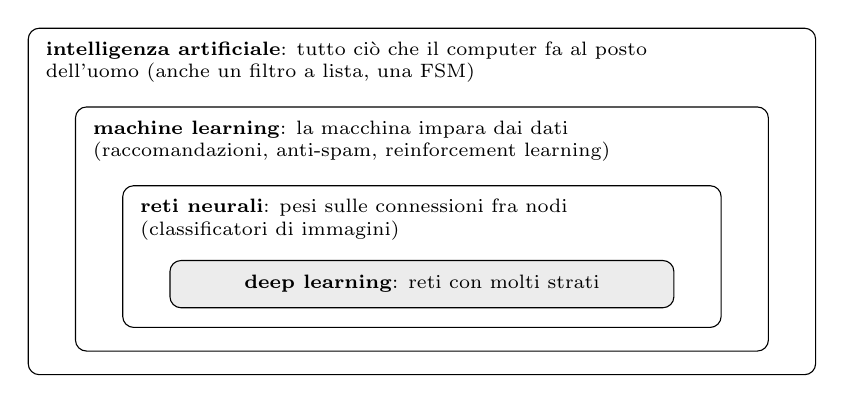
\begin{tikzpicture}[font=\scriptsize]
  \draw[rounded corners] (0,0) rectangle (10,4.4);
  \node[anchor=north west, align=left] at (0.1,4.35) {\textbf{intelligenza artificiale}: tutto ciò che il computer fa al posto\\dell'uomo (anche un filtro a lista, una FSM)};
  \draw[rounded corners] (0.6,0.3) rectangle (9.4,3.4);
  \node[anchor=north west, align=left] at (0.7,3.35) {\textbf{machine learning}: la macchina impara dai dati\\(raccomandazioni, anti-spam, reinforcement learning)};
  \draw[rounded corners] (1.2,0.6) rectangle (8.8,2.4);
  \node[anchor=north west, align=left] at (1.3,2.35) {\textbf{reti neurali}: pesi sulle connessioni fra nodi\\(classificatori di immagini)};
  \draw[rounded corners, fill=gray!15] (1.8,0.85) rectangle (8.2,1.45);
  \node at (5,1.15) {\textbf{deep learning}: reti con molti strati};
\end{tikzpicture}
\caption{La gerarchia dell'intelligenza artificiale come la mostra la slide:
ogni insieme è contenuto nel precedente. Ricostruzione schematica.}
\label{p5:fig:ia}
\end{figure}

\subsection{La macchina a stati finiti}

Nei videogiochi basta spesso una cosa molto semplice: la \textbf{macchina a
stati finiti} (FSM, \emph{finite state machine};
figura~\ref{p5:fig:fsm}). Si pensi al classico gioco di ninja, tipo
\emph{Tenchu}, con le guardie che fanno la ronda:
\begin{itemize}
  \item lo stato di \textbf{patrolling}: la guardia va in giro;
  \item quando il giocatore è abbastanza vicino, passa in \textbf{follow}: lo
        rincorre;
  \item quando è a distanza d'attacco (che dipende dall'arma: con un fucile può
        attaccare da lontano), passa in \textbf{attack};
  \item se il giocatore si allontana, torna in follow e lo insegue; se si
        riavvicina, torna in attacco; se sparisce, o se la guardia lo ha
        ucciso, torna in patrolling.
\end{itemize}
Il patrolling si può variare: se il giocatore è in modalità \emph{stealth}, è
come se il raggio di visione della guardia fosse più stretto; se il giocatore
spara, il raggio diventa di 360 gradi, perché la guardia ha sentito un rumore e
si gira in tutte le direzioni. Si adatta al tipo di gioco.

\begin{figure}[htbp]
\centering
\begin{tikzpicture}[>=Stealth, font=\small, node distance=2.8cm,
  st/.style={draw, circle, minimum size=1.6cm, align=center, font=\scriptsize}]
  \node[st] (p) {patrolling};
  \node[st, right=of p] (f) {follow};
  \node[st, right=of f] (a) {attack};
  \draw[->] (p) to[bend left=20] node[above, font=\scriptsize] {player vicino} (f);
  \draw[->] (f) to[bend left=20] node[above, font=\scriptsize] {a distanza d'attacco} (a);
  \draw[->] (a) to[bend left=20] node[below, font=\scriptsize] {si allontana} (f);
  \draw[->] (f) to[bend left=20] node[below, font=\scriptsize] {sparito} (p);
  \draw[->] (a) to[bend left=45] node[below, font=\scriptsize] {player ucciso} (p);
\end{tikzpicture}
\caption{La macchina a stati finiti della guardia, come nell'esempio della
slide. Ricostruzione schematica.}
\label{p5:fig:fsm}
\end{figure}

È ``una cosa stupidissima che facciamo al primo anno'', ma è la base di un
comportamento, ed è molto potente. Per gli studenti di programmazione,
aggiunge Fattori, è interessante perché una volta capito come funziona una
FSM, ``tutti gli altri sistemi, anche quello di Unreal, che può sembrare più
complicato, sono questo''\footnote{Semplificazione: i \emph{behavior tree} di
Unreal sono una struttura diversa da una FSM, anche se i concetti di base
(stati, condizioni, transizioni) si trasferiscono.}. E i ruoli
\textbf{junior} si aprono facilmente su questi argomenti: Rockstar, subito
dopo l'uscita di \emph{Red Dead Redemption 2}, assumeva tranquillamente junior
gameplay programmer sulla parte di IA. L'\textbf{AI programming} rientra in
genere nella grande branca del gameplay programming, ed è facile trovare
lavoro come junior AI programmer, ``perché tanto è una FSM, è sempre quello'':
è un ottimo punto d'ingresso nel tripla A. Ed è anche la parte più divertente
(i due relatori scherzano: uno ha fatto i bot del gioco dell'altro; ``potrei
dire a Claude: migliorami questa cosa?'' ``No, lo voglio fare io'').

\subsection{Il machine learning nei giochi}

Perché si usa il machine learning? Per far imparare al computer una cosa,
come muovere un personaggio, invece di dirgliela, perché certe volte è molto
difficile. In un gioco di auto la macchina deve andare dritta, curvare in
tempo, non andare addosso agli altri. È più facile farla partire e dirle: se
vai a sbattere contro il muro è male, se non ci vai è bene. È il
\textbf{reinforcement learning}: la macchina va dritta e sbatte, riparte;
alla seconda generazione capisce a caso che sterzando a sinistra, se il muro è
a destra, non lo colpisce, quindi sterza tutta a sinistra e va nel muro di
sinistra; piano piano capisce quando sterzare, quanto prima, e fa un percorso
da sola; con le altre auto impara più o meno a evitarle, magari a sorpassare.

Ma nei giochi il machine learning si usa di rado. Nel gioco di uno dei
relatori, \emph{Slowly Sliding Duck Simulator}, in uscita ``il 29'', i bot non
sono fatti con il machine learning: seguono dei \textbf{percorsi} e usano dei
\emph{raycast} per capire se sono vicini al bordo (se sono vicini al bordo
destro, ruotano a sinistra). L'unico difetto, per un gioco del genere
accettabile, è che si vanno addosso. Anche i giochi di auto si basano su una
FSM: hanno i tracciati del percorso ottimale e cercano di seguirli il più
possibile (``in un gioco di Formula 1 non penso che le Ferrari vadano addosso
alle McLaren'' ``Oddio, potrebbe essere realistico''); una FSM un po' più
dinamica, perché ci si deve aspettare di tutto, con molte ``tecnichette''.

Anzi, la differenza fra una \emph{self-driving car} reale e quella di un
videogioco è che nel gioco il problema è spesso \textbf{renderla un po'
stupida}: ``è un attimo farla mega, mega forte''. Un bot sa tutto: dove sei,
quanta energia hai, quanto inclinarsi per colpirti. Quindi va reso più debole:
prima di una curva, a volte frena troppo presto o troppo tardi, e va fuori.
Nell'altro gioco del relatore, un ``1, 2, 3, stella'', i bot vanno
\emph{nerfati}: al verde partono, al giallo si fermano, al verde ripartono;
bisogna dar loro un ritardo maggiore, se no sono troppo forti.

Anche il filtro che mette il muso di cane sul volto è machine learning:
bisogna capire che quella è una faccia, dove sono gli occhi, il naso, la
testa. E un \textbf{classificatore}: gli si dà un'immagine e dice che cos'è,
con la probabilità che sia un cane, un gatto o un uccello; ormai lo si fa in
tempo reale, con una webcam.

% ---------------------------------------------------------------------
\section{Il network programmer}
\label{p5:sec:network}

(``Matteo, vai un po' veloce, se no non ci facciamo fare domande''.) Il
network programmer si occupa del \textbf{multiplayer}, se c'è. L'esempio
classico è Internet: col computer si chiede qualcosa a Google e il server
restituisce una pagina HTML; il server di Facebook comunica con il cellulare e
gli manda i dati dell'app. In un gioco con una \textbf{lobby} bisogna sapere
quanti player ci sono, chi sono, come si chiamano: si comunica con un server,
che avrà un database, e che restituisce le informazioni (``waiting for
players'').

Poi c'è la gestione dei \textbf{pacchetti}: per ogni altro player arrivano le
informazioni su dove sta, come è ruotato e con quale velocità si muove. Se i
pacchetti non arrivano, lo si vede andare da qui a qui e poi direttamente là:
è il \textbf{lag}. La slide mostra la \emph{lag compensation}\footnote{Quella
descritta, cioè stimare la posizione di un giocatore a partire dall'ultima
posizione e velocità note, si chiama più propriamente \emph{dead reckoning}
o estrapolazione (\emph{client-side prediction} quando riguarda il proprio
personaggio); con \emph{lag compensation} si indica di solito la tecnica, lato
server, che ``riavvolge'' lo stato del gioco per verificare i colpi.}: avendo
anche la velocità del player, quando si perdono i pacchetti si suppone che,
se andava a destra a 45 gradi, sarà più o meno in quella posizione; quando le
informazioni tornano, il player è più o meno dove previsto. A meno che non
abbia sterzato subito dopo la perdita dei pacchetti.

I giochi online, aggiunge Fattori, \textbf{laggano per definizione}: c'è
sempre un tempo di risposta, perché l'informazione deve partire dal computer
di un giocatore, arrivare al server e tornare all'altro. Per questo si tende
sempre a prevedere più o meno dove sarà il giocatore, per creare un movimento
fluido. ``Il movimento fluido che vedete nei giochi online non è mai vero, è
sempre finto''.

% ---------------------------------------------------------------------
\section{Che cosa fa, in sintesi, il programmatore}
\label{p5:sec:ruolo}

Al programmatore vengono dati tutti gli asset, 2D o 3D; lui li mette in un
progetto, in un motore (Unity, Unreal o un motore fatto in casa) e \textbf{fa
funzionare il gioco}: implementa il gameplay, i suoni, quanto danno fa una
spada. Ovviamente chi gli dice quanto danno fa la spada è il \textbf{game
designer} (capitolo~\ref{p2:cap:gamedesign}); chi fa i suoni è il musicista o
il sound designer; chi scrive la storia è il \textbf{narrative designer}
(capitolo~\ref{p3:cap:narrative}).

% ---------------------------------------------------------------------
\section{Come si comunica con un programmatore}
\label{p5:sec:comunicare}

È ``un punto molto importante'', soprattutto per i non programmatori presenti,
e lo tratta Fattori.

\subsection{Essere specifici, coprire tutti i casi}

Il lavoro del programmatore è molto, molto tecnico, e ha bisogno di
\textbf{informazioni chiare}. È bene sentire la sua opinione, ma quando gli si
comunica qualcosa bisogna essere \textbf{estremamente specifici}: ``non perché
sono stupidi i programmatori, anche se alcuni posso confermare''. A Fattori è
successo tante volte che un programmatore arrivasse ``incazzato a merda'' con
il game designer perché gli aveva dato un GDD, o un documento su una
meccanica, in cui mancava tutta una serie di informazioni fondamentali.

Quando si spiega come si vuole implementare una meccanica, o ci si fa aiutare
dal programmatore (che, se è bravo, ragiona già sui \textbf{casi limite}: ``ma
se c'è questa cosa e c'è quest'altra, cosa deve succedere?''), oppure si
coprono da soli \textbf{tutte le casistiche possibili}; o, meglio ancora, la si
sviluppa insieme. Fattori non fa più il programmatore ogni giorno (ha un altro
ruolo nella sua azienda), ma parlando con il suo programmatore vede che questo
ragionamento viene subito, ``e ce l'ho anch'io dietro la capoccetta'': ``devo
fare danno a un tizio. Ma se il tizio ha lo scudo, che succede? Prende meno
danno?''. Altrimenti il programmatore resta potenzialmente perso: uno
``smagato'' magari trova una soluzione e la propone; uno studente,
realisticamente, si impappina, e lo si mette in difficoltà.

\subsection{Che cosa pretendere: la fattibilità}

Da un programmatore si deve pretendere una \textbf{stima di fattibilità}: una
delle domande da fargli è ``è fattibile?''. Che cosa vuol dire fattibile?
``Mi piace sempre dire che in programmazione si può fare tutto, l'importante è
quanto tempo c'è a disposizione''. La fattibilità dipende da due cose:
\begin{itemize}
  \item il \textbf{tempo}: ci si deve aspettare risposte come ``per questa cosa
        ci metto una settimana, per questa due settimane'';
  \item la \textbf{tecnologia preesistente}: se i nemici sono codificati per
        muoversi in due dimensioni, su un piano, non si può chiedere un piano
        rialzato, perché vorrebbe dire riscrivere tutta la parte dei nemici.
        ``È un caso estremo'', ma spesso ``non fattibile'' vuol dire solo che
        ci vuole tantissimo tempo.
\end{itemize}
Dal prossimo anno si lavorerà con i programmatori, con delle scadenze, e il
programmatore dovrà saper dire: ``questa cosa non è fattibile nelle
scadenze''. È il \textbf{metodo di comunicazione standard}: i designer devono
comunicare in maniera chiara e diretta, coprendo tutte le casistiche; i
programmatori devono spiegare come intendono implementare, dire che cosa gli
serve (magari informazioni che non si erano previste) e dare delle
\textbf{tempistiche}.

\subsection{Team grandi e team piccoli}

In un grande studio il programmatore fa il programmatore: Fattori non faceva
gameplay programming, quindi ``di quello che dicevano i designer non mi
fregava niente''; negli ultimi tempi parlava soprattutto con gli animatori.
In un team molto grande c'è meno comunicazione: spesso arriva il team lead e
dice ``devi fare questo''. Nei team molto piccoli ce n'è tanta, e spesso i
programmatori hanno idee e una visione loro sul design: quindi dategli le
informazioni, ``ma non abbiate paura di chiedergli il loro parere, anche
artistico''.

\subsection{Un esempio: gli oggetti ``nuovi''}

Un esempio pratico, ``successo ieri'': il nuovo mockup del \emph{market} di un
gioco, in cui si possono vedere gli oggetti in vendita o gli oggetti nuovi,
con l'etichetta \emph{new}. Ma che cosa vuol dire ``nuovi''? Sono gli ultimi
$n$ inseriti, che restano nuovi finché non se ne mettono altri? E allora
quanti sono? Oppure è nuovo un oggetto inserito da meno di due settimane? Fa
molta differenza su come lo si implementa. Non è cattiveria né mancanza di
elasticità mentale: per dire a una macchina ``mostrami solo gli oggetti
nuovi'' bisogna dirle \textbf{che cos'è un oggetto nuovo}, ``la macchina non
lo sa''. Le domande dei programmatori possono sembrare pedanti (``un oggetto
nuovo è uno che non è vecchio''), ma chiedono solo: qual è la soglia?

\subsection{Con i 3D artist, e con tutti}

Fattori fa questo discorso per game designer e narrative designer, perché con
i \textbf{3D artist} è diverso: sono ``forse più tecnici dei programmatori'',
e storicamente sono sempre andati d'accordo, ``a meno che non sbagliate il
pivot, e allora vi fate odiare a morte dal programmatore che deve ricentrare
quell'oggetto. Questa è una minaccia''. La lingua di un 3D artist è molto più
comprensibile per un programmatore; anche se il lavoro ha una componente
artistica non indifferente, è molto tecnico, e i 3D artist usano molti più
software dei programmatori (``noi abbiamo il nostro bellissimo ambiente di
sviluppo, il nostro engine, e siamo felici così''). Con designer e narrative,
invece, può esserci incomprensione: bisogna essere sempre molto chiari.

E soprattutto: \textbf{nessuno è nemico di nessuno}. Si è tutti nello stesso
team e si sta cercando di portare avanti un videogioco. Se si dà per scontato
che il programmatore non vi odia (``a meno che non sia uno stronzo, e questo ce
ne accorgiamo in tempo zero''), ci si può parlare tranquillamente.

% ---------------------------------------------------------------------
\section{Le domande}
\label{p5:sec:domande}

\subsection{Comincio da zero, a trent'anni: come mi preparo?}

Uno studente, arrivato in ritardo (``si è sciolto tutto il ghiaccio del
frigo, un disastro''), ripete la domanda fatta il giorno prima al docente di
narrative: è iscritto a programmazione, parte \textbf{completamente da zero},
senza aver mai scritto una riga di codice, ha 30 anni e già esperienza
lavorativa in altri settori: progettava ascensori in AutoCAD. Chironi lo
rassicura: non sarà l'unico, ``non è che sono tutti ingegneri e scienziati gli
altri, sono quasi tutti diciannovenni che non hanno mai programmato''. ``A 30
anni magari è tardi per iniziare a fare parkour, ma per programmare no'':
anzi, avrà una \emph{forma mentis} più seria di un ragazzo più giovane. E ``sei
ancora molto più giovane dello studente più anziano che abbiamo avuto''.

Come prepararsi? Basta \textbf{seguire le lezioni e fare domande in classe}.
Lo dice a tutti alla prima lezione: non siamo alle superiori. Chi viene e paga
si presume che voglia fare questo lavoro, quindi \textbf{tutto quello che
viene spiegato serve}, ``più o meno tutti i giorni, per trovare lavoro e per
lavorare''. Non è il liceo, dove ``c'è il latino, ma che me ne frega del
latino, di filosofia, di Schopenhauer'' (``poi magari vi interessa più da
vecchi''): non si lasciano indietro cose, come ``la perifrastica passiva''. A
fine lezione bisogna aver capito ``non dico il 100\%, ma almeno un 85\%''; e
se qualcosa non torna, la si riguarda a casa, perché le lezioni sono
registrate e il giorno dopo si possono rivedere. Certe cose, come la
collisione fra cerchio e rettangolo, sono difficili da capire mentre uno te le
spiega: ``prendetevi del tempo a casa per riguardarle da soli, vedrete che da
soli ci arrivate meglio''.

\textbf{Non restare mai indietro}. C'è chi dice ``vado via un mese'', ``bello
per te'', e poi viene bocciato male: come si recuperano nove ore di lezione a
settimana per un mese? Se si resta indietro, si sfrutta il \textbf{tutor}. E
le classi online dovrebbero essere più collaborative (quest'anno
programmazione è solo online): fate domande. Un aneddoto: c'era un ragazzo
molto bravo, che veniva sempre (a volte in aula c'era solo lui, ``anche se gli
altri erano iscritti in modalità campus''), rispondeva sempre. Al secondo
esame ``fa un troiaio'', arriva tardi. Ma il docente, conoscendolo e sapendo
quanto sapeva, lo considera comunque preparato. Invece di ``un tizio random in
chat, sempre mutato, che non so chi è e non risponde mai'', se fa male
l'esame, ``per me non sa nulla''. Quindi rendiamo la classe più umana.

\subsection{Non basta il 100\%: serve la fame}

Fattori ``ci mette il carico da dodici'', perché lo studente sta facendo un
percorso molto simile al suo prima dell'accademia: vuole cambiare
completamente vita, e lavorare nei videogiochi o anche nel cinema, ``nel
fantastico mondo dell'intrattenimento''. ``Non basta il 100\%, purtroppo:
devi farti venire la \textbf{fame}''. La caratteristica comune di tutti quelli
usciti da AIV che hanno fatto videogiochi è che hanno fame di farli, ``un
bisogno fisico''. Non si viene in accademia per fare il compitino: quello basta
per essere competenti. Ma, come diceva Chironi, tutti quelli che imparano a
programmare a un certo punto vogliono fare videogiochi. Se si esce da AIV con
le competenze, ma senza essersi spaccati la schiena, senza essere andati alle
fiere ``perché non t'andava'', si viene battuti ai colloqui da chi ha le stesse
competenze, ha fame, ed è andato agli eventi e ha conosciuto persone che già
fanno questo lavoro.

``Il game dev è una piccola famiglia: una volta che sei dentro, sei dentro. Il
problema è entrare''. C'è un po' di \emph{gatekeeping}, ma non per cattiveria:
``se devo assumere te o uno che vedo tutti i mesi a tutte le fiere, è chiaro
che vado su quello che già vedo'', perché mentalmente è già nell'ambiente.
Primo consiglio, per tutti: \textbf{fatevi tutte le fiere} (la First Playable
di Firenze, e qualsiasi altra a portata di mano, purché si sappia che ci sia
almeno uno sviluppatore); prendete contatti; il networking è fondamentale.

E poi fate videogiochi. Al terzo anno Fattori lavorava mentre frequentava
AIV, ``coadiuvato dal fatto che era pandemia'': la mattina lavorava, il
pomeriggio seguiva le lezioni, e da quando staccava fino all'ora di andare a
letto faceva videogiochi. ``Vi dovete spaccare la schiena'': nel tempo libero
magari una partita la si fa, ma il resto è dedicato a fare videogiochi. ``So
che è brutto, so che è lontano dall'etica lavorativa in cui ci stiamo
muovendo, però l'ambiente è competitivo''. Non serve essere geni per
frequentare AIV o fare i programmatori, le cose vengono spiegate in modo che
tutti ci arrivino; ma fra uno che è a 90 e uno che è a 95, ``assumerò quello a
95, a meno che non sia un serial killer, e si capisce dallo sguardo''. Come in
un'accademia di recitazione: quanti diventano attori? Quelli che sono stati a
casa a provare e riprovare.

Chironi aggiunge che a programmazione dice sempre ``basta che abbiate
capito'', mentre in 3D art\footnote{Nella trascrizione ``Morini, 3D Art, dice
sempre'': non è chiaro se il riferimento sia ad Andrea Morini
(capitolo~\ref{p1:cap:devdays}) o al docente di 3D art
(capitolo~\ref{p6:cap:3d}).} si dice sempre che bisogna stare a casa a rifare,
rifare, rifare, perché è una cosa più meccanica: ``dovete fare mille modelli
per imparare bene''. Fattori precisa che \textbf{aver capito non vuol dire
aver visto tutti gli edge case}: come diceva Niels Bohr, un esperto è una
persona che ha commesso tutti gli errori possibili in un determinato ambito.
Quindi bisogna buttarsi e provare a fare un videogioco con le competenze di
base. Il suo gruppetto in accademia (per caso, gli unici tre di quell'anno che
hanno trovato lavoro nei videogiochi: uno ora è in Blizzard, lui ha la sua
azienda, un altro ha fatto un gioco\footnote{Nella trascrizione ``Dinopath'':
il titolo non è verificabile.}) era fatto dei tre che, staccando dalle
lezioni, si mettevano a fare videogiochi con le poche competenze che avevano.
Ogni volta che sbloccavano una competenza, capivano come implementarla nel
gioco; a volte, sapendo che ci sarebbe stata una lezione su un argomento (il
\emph{pathfinding}, per esempio), cominciavano a studiarlo prima perché
serviva al gioco. Così arrivavano a lezione conoscendo già le basi, e la
lezione rifiniva concetti che avevano. ``Questo è un po' estremo, eravamo i
nerd sfigati della situazione'', ma è il concetto di fame: ``io faccio
videogiochi perché ho bisogno di fare videogiochi''; potrebbe tranquillamente
fare software per i dipendenti dell'ENEL. Anche Chironi (``ho fatto molto di
peggio in vita mia''\footnote{Segue una battuta incomprensibile nella
trascrizione (``ho potuto rispondere alle mail di me contro te'').}).

\subsection{L'aneddoto di Vampire Survivors}

Chironi racconta un aneddoto. Il primo anno che insegnava aveva tre studenti,
e uno era Luca Galante\footnote{Nella trascrizione ``Luca Pieracci, che ora si
chiama Luca Galante'': il cambio di cognome non è verificabile.}, l'autore di
\emph{Vampire Survivors}. Si dice: ``si è svegliato una mattina ed era
milionario''. Ma intanto si era trasferito a Londra, lavorava da McDonald's e
faceva videogiochi nel tempo libero; poi ha trovato lavoro nel settore delle
slot. Tornava a casa alle sei di sera, andava a letto alle sette, si svegliava
alle tre di notte per programmare fino alla mattina, e poi andava al lavoro.
È riuscito a fare \emph{Vampire Survivors}, prima per mobile, poi per PC e
Steam\footnote{L'ordine è invertito: \emph{Vampire Survivors} è uscito prima
su PC (itch.io e poi Steam, in accesso anticipato, nel dicembre 2021), e le
versioni mobile sono arrivate nel 2022.}, ``e poi ha fatto i soldoni''. Si è
impegnato ``come un cane''; e ha avuto anche fortuna, perché tanti fanno
giochi più o meno belli e poi hanno quattro recensioni (``tre recensioni in un
gioco del 2018: mamma mia, da sviluppatore mi sento male'').

\subsection{Come sono strutturati gli esami?}

A differenza degli altri corsi, a programmazione \textbf{ci sono esami}
(si veda anche il capitolo~\ref{p1:cap:devdays}). Come funzionano? ``Gli esami
sono fatti per distinguere gli uomini e le donne dalle bestie'', scherza
Chironi; non è ``ho la media del 17,56, sono bocciato''. Servivano prima perché
l'accademia era riconosciuta con l'Università Mercatorum, ``ora non è più
riconosciuta, che io sappia''\footnote{Così il relatore; l'informazione non è
verificabile dalla trascrizione.}; e servono perché, essendoci una modalità
online, ci sono persone di cui il docente ``non sa neanche che faccia abbiano''
e che magari non vengono alle lezioni: perché dovrebbero passare al secondo
anno? Devono dimostrare di essere arrivati al livello richiesto.

Al \textbf{primo anno} ci sono:
\begin{itemize}
  \item \textbf{due scritti}, online con Google Forms, a crocette o a risposta
        aperta;
  \item \textbf{tre progettini} da consegnare, principalmente video: il
        docente guarda il video del gameplay e, se è fatto come ha chiesto, va
        bene.
\end{itemize}
È più come le superiori che come l'università: se al primo esame si ha il
dentista, non c'è un altro appello; bisogna dimostrare la preparazione con
tutto quello che si fa dopo. Conta più il secondo esame del primo: se al primo
si prende 10/30 e al secondo 28, si presume che alla fine dell'anno si sia
capito tutto quello che c'era in mezzo. Per chi è ``mezzo e mezzo'' c'è anche
a settembre uno scritto e un po' di orale. Ma è raro: di solito chi viene
bocciato male ha fatto una sola cosa in tutto l'anno, o zero; gli altri,
bene o male, ce la fanno.

Al \textbf{secondo e al terzo anno}, con Fattori, è diverso: ``gli esami non
servono a me''. Le sue lezioni sono molto interattive, e durante l'anno vede
tutti lavorare e interagire: sa benissimo qual è il livello di ciascuno. Gli
esami servono agli studenti. ``Non mi serve che mi prendiate 30, perché nella
maggior parte dei casi, se mi prendete 30, avete aperto Claude e l'avete fatto
fare a lui'': gli è successo tutti gli anni, da quando è uscito ChatGPT. ``Non
è che diventate chirurghi e mettete una patata nel cervello di qualcuno perché
vi ho preparato male io'': se si imbroglia e non si sanno le cose, non si
troverà lavoro, ``e sarete quelli che la coltivano, quella patata'' (``che
comunque non è banale, anzi, forse è una professione più sicura al giorno
d'oggi''). Gli è capitato di avere studenti che alla lavagna non sapevano
scrivere un'istruzione e che all'esame prendevano 28-30, mentre altri più
fluenti nel codice prendevano 24-26: ``lì è chiaro''. Con la modalità mista,
online e in presenza, diventa complicato; i suoi esami sono in genere a
crocette, ``proprio perché serve a voi''. Lui sa come scrivete codice, ``che
alla fine è quello che mi interessa''. Nessuno dei due è ``un grande fan degli
esami'': c'è anche chi è bravo e all'esame ``si caca addosso''. ``Ricordatevi
che siamo umani: non vi daremo mai un voto basato su un algoritmo, nonostante
siamo programmatori''.

\subsection{E l'intelligenza artificiale?}

L'IA è nel programma, dice Chironi, ma ``è come se in un corso di cucina vi
insegnassi a ordinare la pizza su Just Eat'': bisogna sapere che esiste, ma
saper fare le cose da zero. Fattori mostrerà Claude, i vari agenti; ma la base
di preparazione serve, perché la macchina ``non è ancora smaliziata come
l'essere umano'' e a volte propone soluzioni strane. E qualsiasi campo si
scelga, dopo tre anni non si esce ``al top'': si è bravissimi come junior, ma
bisogna continuare a studiare e a fare pratica.

\subsection{Un non programmatore può fare un gioco per esercizio?}

Uno studente chiede come muoversi, da non programmatore, per fare un
videogioco per pratica: Unreal? Blueprint? Sì, finché ci sono; oppure, suggerisce
Fattori, una cosa molto utile: si paga l'abbonamento a Claude e si impara una
skill in più, \textbf{comunicare con un'intelligenza artificiale}. A
programmazione lo si fa al secondo anno: una delle prime lezioni sarà proprio
su come si parla con l'IA ``in modo da non svalutare il vostro lavoro, le
vostre competenze''. Al primo anno, aggiunge Chironi, c'è un progettino con una
parte difficile per cui il docente dice ``se volete, usate l'IA'', perché è
interessante cominciare a usarla per fare una singola cosa di un progetto
proprio.

\subsection{Libri consigliati}

\begin{itemize}
  \item \emph{Game Programming Patterns}\footnote{Di Robert Nystrom (2014); il
        relatore lo chiama prima, lapsus, ``Game Design Patterns''.}: va bene
        per qualsiasi linguaggio e presenta i \textbf{pattern di
        programmazione}, cioè come strutturare un pezzo di codice per fare cose
        comuni: il singleton, il pooling, il component pattern, cose che si
        studieranno durante l'anno. Va bene anche per un neofita. È un libro
        tecnico, ma si trova gratis in HTML sul sito dell'autore.
  \item Libri tecnici sui linguaggi i relatori non li consigliano mai,
        ``perché vengono aggiornati''. Se proprio, \emph{Effective Modern
        C++}\footnote{Di Scott Meyers (2014).}, ma interessa dal terzo anno in
        poi, ed è argomento di corso.
  \item \emph{Blood, Sweat, and Pixels}\footnote{Di Jason Schreier (2017). Il
        relatore cita fra i giochi trattati \emph{Terraria}, che però non è fra
        i capitoli del libro (che racconta, fra gli altri, \emph{Pillars of
        Eternity}, \emph{Uncharted 4}, \emph{Stardew Valley}, \emph{Diablo
        III}, \emph{Shovel Knight}, \emph{Destiny}, \emph{The Witcher 3});
        \emph{Uncharted} invece c'è.}: una lettura leggera, non tecnica, sui
        retroscena dello sviluppo di molti giochi famosi, scritta da un
        giornalista che intervista gli sviluppatori. ``Interessante per tutti,
        anzi, forse per i programmatori ancora meno''; ``vi fa aprire gli occhi
        su un sacco di cose che succedono nell'industria''.
\end{itemize}

\subsection{Serve un'intelligenza più pratica che artistica?}

Lo stesso studente chiede: se non serve necessariamente la matematica, serve
almeno un'intelligenza più pratica che artistica? ``Dipende''. Chironi è sempre
stato molto portato per la programmazione e ``zero per la matematica'': molte
cose le ha imparate dopo, usandole, ``ah, è per questo che serve''. E per
questo si considera bravo a spiegarla: come nei film anni Ottanta, dove ``per
prendere il killer pazzo usavano il poliziotto pazzo'', la matematica la
insegna meglio chi ha avuto difficoltà a capirla; ``ho insegnato a cani e porci
la trigonometria''. Serve però una mente \textbf{analitica}: non le formule, ma
``se vedi due numeri e impazzisci, è un problema''; ``se non ti piace il
sudoku, è un indizio''. Un programmatore è uno a cui piace \textbf{decifrare}
le cose: lui da piccolo cercava di decodificare i file di salvataggio dei
giochi. ``Se ti fa schifo vedere il codice, è un problema''.

Fattori aggiunge un test: guardare un tutorial di Unity, anche il primo, quello
in cui si preme avanti e la pallina si muove, e vedere la corrispondenza fra
quello che succede sullo schermo e il codice scritto. ``Se vi affascina,
avete buone chance che la programmazione vi vada bene''. E il lavoro del
programmatore, di base, è prendere un problema che si presenta in forma
\textbf{descrittiva} (``come faccio a fare questa cosa?''),
\textbf{decomporlo} e costruire una soluzione passo dopo passo per la
macchina: il ``brutto concetto'' di \emph{problem solving}.

A questo punto Chironi deve andare (``per chi è iscritto, ci vediamo a lezione
su Zoom; per gli altri, buona fortuna''), e Fattori prosegue da
solo\footnote{L'attribuzione è dedotta dal contesto: è Chironi che insegna al
primo anno, online; Fattori aveva detto che a lezione non lo si sarebbe più
visto se non in control room.}.

\subsection{Esistono programmatori che lavorano da soli?}

Sì\footnote{Nella trascrizione la domanda è ``esistono programmatori che
lavorano su Resident Evil?'': dal contesto, ``da soli'', senza un team.}, ma in
genere hanno anche altre competenze. L'amico di Fattori che ora è in Blizzard
per un periodo è stato sviluppatore solitario (non è riuscito a pubblicare
nulla, perché poi ha trovato lavoro), ma aveva competenze di 3D art, e infatti
ora fa il technical artist. È fattibile: ``basta un minimo di competenza in
pixel art''. Ma Fattori lo sconsiglia, ``perché non è divertente''. Ha sempre
visto i videogiochi come uno \textbf{sforzo di gruppo}: si possono fare anche
da soli, con ottimi risultati, ma il punto di forza dei videogiochi è che
uniscono competenze diverse, e competenze diverse vogliono dire persone
diverse. ``Mi piace pensarla come una grossa famiglia felice del game dev''
(``poi alcuni si odiano fra loro, ovviamente ci sono anche persone che odio in
questa industria''), in cui si collabora ``per creare qualcosa di enormemente
più grande di noi''.

\subsection{Come interagisce un 3D artist con un programmatore?}

È molto più facile, perché fino a un certo punto si parla la stessa lingua. Il
punto di contatto è quando il modello è pronto e va messo in engine: il 3D
artist dà le UV, le normal, l'albedo, tutte le mappe, e il programmatore le
prende e le piazza dove devono andare (``il programmatore sa che cos'è
l'albedo''). Lo step con più attrito è la \textbf{resa finale}: il modo
migliore è farla insieme. Il programmatore mette il modello in engine (o
l'artista impara a farlo, ``sono due tasti''), e si lavora insieme per arrivare
all'effetto estetico che l'artista aveva in mente.

A seconda del livello (in tre anni di accademia è difficile arrivarci) si discute poi
di \textbf{ottimizzazione}, in fase di pianificazione del
modello: il \emph{polycount}. Non è un ``ti do queste informazioni perché mi
serve così'': è una discussione, perché il polycount cambia a seconda
dell'importanza del modello. ``Ti vedo questo modello con 10 milioni di
poligoni''; il programmatore: ``no, 10 milioni di poligoni, stronzo''. ``Ok, però
è un modello importante''. ``Va bene, facciamo un milione''. ``Un milione è
ancora un po' tanto, scendiamo un pochino''. Si arriva a una soluzione che abbia
senso per entrambi: una \textbf{discussione costruttiva}.

\subsection{Contano di più i lavori consegnati? E se non si passa un esame?}

Uno studente ha sentito che, per passare l'anno, contano di più i lavori
consegnati. Ci sono degli \emph{assignment} da consegnare a fine anno, molto
importanti perché pratici; ma, come spiegato, è un \textbf{percorso}: non si
guarda l'esame consegnato e finisce lì. E se non si passa un esame? ``Non hai
passato l'esame, pace'': lo si segna sul tabellone con i voti. Banalmente, ci
si mette sotto a studiare: non passare un esame è un buon momento per capire
che si deve rivedere un argomento, fare un passo indietro, riguardarsi tutto
quello che manca e recuperare all'esame successivo. ``Se hai lavorato bene,
probabilmente lo passi''.

\subsection{Si può saltare un anno?}

Fattori ha tempo per un'ultima domanda (deve andare a una riunione). Filippo
chiede se si può saltare un anno. Se ne parla con il docente dell'anno e con
il direttore dei corsi, ``ovviamente Andrea''\footnote{Con ogni probabilità
Andrea Morini (capitolo~\ref{p1:cap:devdays}).}: si fa un colloquio specifico
e potenzialmente un esame (un'idea sarebbe far partecipare a un esame in
particolare). Ma Fattori lo \textbf{sconsiglia}: arrivato in accademia sapeva
già programmare e gli avevano proposto di saltare il primo anno; l'ha fatto lo
stesso, e ha coperto tante lacune. L'anno che ha senso saltare è il primo,
perché magari si hanno già competenze di programmazione, ma difficilmente di
programmazione di videogiochi. Saltare il secondo vuol dire perdersi Unity e
Unreal e passare al terzo, in cui non si fanno: al terzo anno si fa
programmazione a basso livello, si parte dall'Assembly, si fa il C, il C++, e
``una robetta di Unreal'' giusto per restare freschi, senza rispiegarlo. Quindi
non lo consiglia mai, a meno di avere, per esempio, una laurea in ingegneria
informatica con una tesi sui videogiochi: allora si può fare solo il terzo
anno, parlandone con il direttore dei corsi e con i docenti di programmazione.

\subsection{La webcam}

Uno studente avvisa che non può accendere la webcam perché gli arriva ``il 6
ottobre''. Nessun problema: online Fattori chiede di solito la webcam accesa
``più che altro perché, guardando i volti, capisco se vi state addormentando''.
In alcuni corsi può essere più importante; qui è solo una questione di
feedback dalla classe. Un altro chiede della tastiera: Fattori ha una
\emph{tenkeyless} (TKL), senza tastierino numerico, e per programmare ``basta
che hai le lettere, i numeri e i punti e virgola''.

\subsection{L'ultimo consiglio: fiere e game jam}

``Ci sono eventi di videogiochi: fateveli tutti''. \textbf{Firenze è
obbligatoria}: farsi vedere alla \textbf{First Playable}, che si tiene a
inizio giugno (``escono poi le date''), ``dove trovate tutti, fondamentalmente''.
E alle varie fiere dove ci sono gli sviluppatori: ``probabilmente mi vedrete
lì, sentitevi liberi di darmi una botta sulla spalla e fare due chiacchiere''.
Tra un mese e mezzo c'è la \textbf{Milan Games Week}: ``lì mi trovate, non
abbiate timore di venirmi a importunare, tanto sono lì ad annoiarmi allo
stand''. (Uno studente propone una lista di eventi: ``la prepariamo,
interessante, ottima idea''.)

E fatevi le \textbf{game jam}. ``Non fate la storia: ho appena iniziato, non
sono in grado''. La prima game jam Fattori l'ha fatta prima di entrare in AIV,
perché voleva fare videogiochi: ``male che va faccio un gioco di merda. Bene, ho
fatto il gioco di merda della mia vita, perfetto, adesso andiamo a fare quelli
belli''. Il ragionamento è questo: \textbf{il primo gioco sarà sempre brutto},
è inevitabile; quindi fatelo il prima possibile, così quello dopo sarà meglio,
e quello dopo ancora. In una jam si sceglie il linguaggio e il motore (Godot,
Unity, Unreal, il proprio motore, ``whatever''). Se ci si va da soli, si trova
un team e si dice ``ragazzi, sto iniziando a studiare, posso unirmi a voi?''.
``Se trovate uno che vi dice: no, vogliamo solo quelli forti, ditemi nome e
cognome che lo vado a menare, perché non ha capito come funziona la game
jam''. La jam è ``più una scusa per passare un weekend a fare videogiochi''.

Il consiglio finale, ``forse il migliore che posso dare a tutti gli ambiti'':
\textbf{non abbiate paura di sbagliare}, perché l'unico modo per imparare è
sbagliare. Magari si finisce in un team di gente forte che dice ``questa cosa,
la prossima volta, falla così perché è meglio'', e si esce con un bagaglio
arricchito. Il gioco che Fattori sta sviluppando ora, quello che porterà a
Milano e che è su Steam, è nato da una game jam: anche questo può succedere.
Ma il modo sbagliato di affrontare una jam è ``devo fare un gioco che poi
continuo, sviluppo, pubblico e ci faccio miliardi''. Il modo corretto è:
\textbf{``vado a fare videogiochi''}. (Si veda anche, sulle jam, la
sezione~\ref{p2:sec:jam}.)
